\begin{figure}[t!]
    \centering

    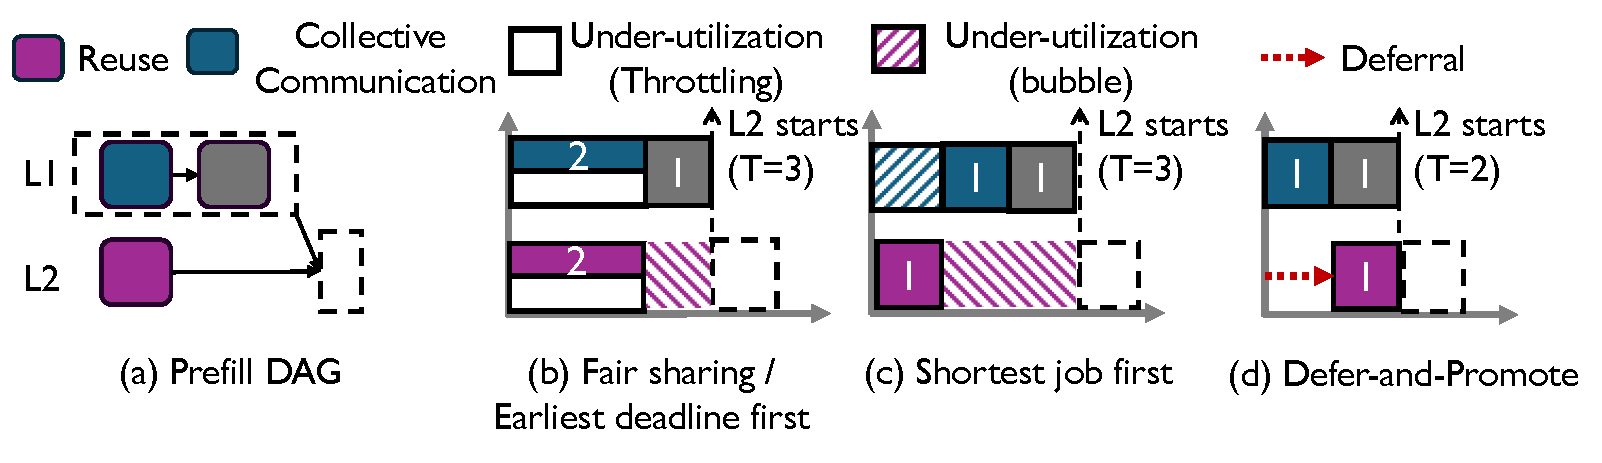
\includegraphics[width=\linewidth]{figures/methodology/IntraContentionExample-A.pdf}
    \caption{\textbf{Comparison of scheduling policies for intra-request contention (ingress).}
    (a) Ingress port contention during Layer-1 execution.
    (b)-(c) FS/SJF/EDF delays the start of Layer-2 ($T=3$).
    (d) The \textit{Defer-and-Promote} strategy advances the Layer-2 start time to $T=2$ (-33\%).}
    \label{fig:meth:intraA}

    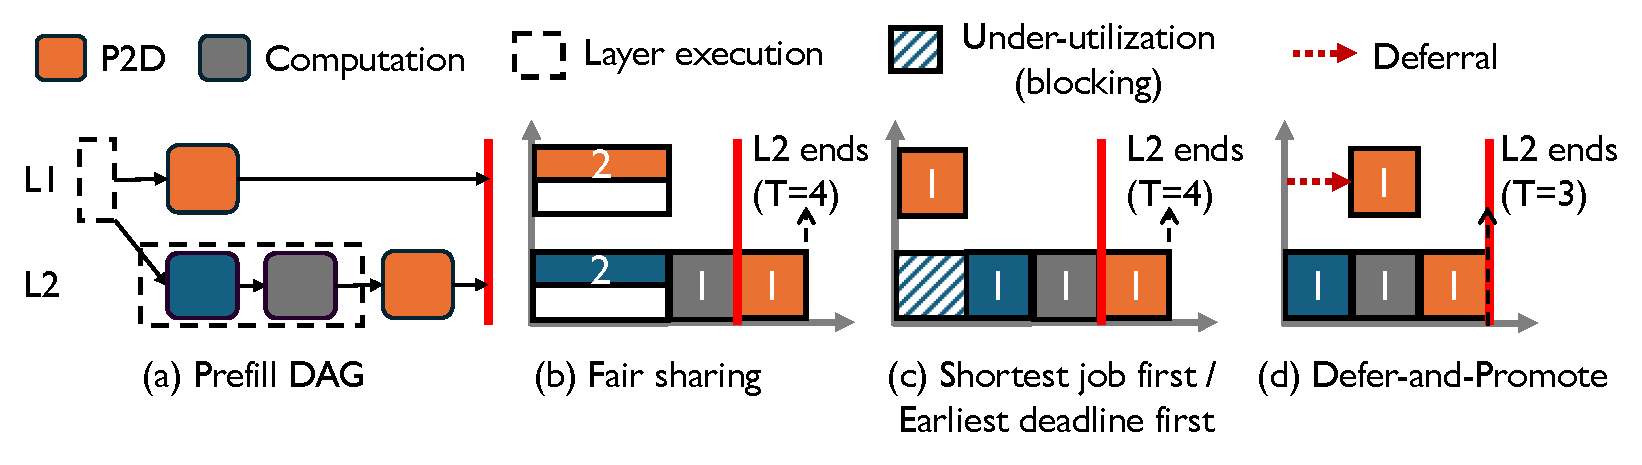
\includegraphics[width=\linewidth]{figures/methodology/IntraContentionExample-B.pdf}
    \caption{\textbf{Comparison of scheduling policies for intra-request contention (egress).}
    (a) Egress port contention during Layer-2 execution.
    (b)-(c) FS/SJF/EDF delays the end of Layer-2 ($T=4$).
    (d) The \textit{Defer-and-Promote} strategy reduces the Layer-2 finish time to $T=3$ (-25\%).}
    \label{fig:meth:intraB}
\end{figure}
